\documentclass[10pt,mathserif]{beamer}

\usepackage{graphicx,amsmath,amssymb,tikz,psfrag,subfigure,bm}

\input defs.tex

%% formatting

\mode<presentation>
{
\usetheme{default}
}
\setbeamertemplate{navigation symbols}{}
\usecolortheme[rgb={0,0,0}]{structure}
\setbeamertemplate{itemize subitem}{--}
\setbeamertemplate{frametitle} {
	\begin{center}
	  {\large\bf \insertframetitle}
	\end{center}
}

\AtBeginSection[] 
{ 
	\begin{frame}<beamer> 
		\frametitle{Outline} 
		\tableofcontents[currentsection,currentsubsection] 
	\end{frame} 
} 

%% begin presentation

\title{\large \bfseries Gaussian Process}

\author{Jiali Lin\\[3ex]
Virginia Tech}

\date{\today}

\begin{document}

\frame{
\thispagestyle{empty}
\titlepage
}

\section{Introduction}
\begin{frame}{Introduction}
\begin{itemize}
    \item We observe some inputs $\bm{x}_i$ and some outputs $y_i$ (i.i.d).  
    \item We assume linear relationships
    \begin{equation*}
        y = f(\bm{x}) = \bm{x}^T \bm{w},  \quad y = f(\bm{x}) + \epsilon, \quad \epsilon \sim N(0, \sigma_n^2)
        %\bm{y} = f(\bm{x}) = \bm{x'w},  \quad \bm{y} = f(\bm{x}) + \bm{\epsilon}, \quad \bm{\epsilon} \sim N(0, \sigma_n^2)
    \end{equation*}
    \item Prior: $\bm{w} \sim N (0, \bm{\Sigma}_p)$.
    \item To make predictions on new input $\bm{x}_*$, we use posterior predictive distribution
    \begin{equation*}
        p(y_*|\bm{x}_*, \bm{X}, \bm{y}) = \int p(y_*|f, \bm{x}_*)p(f|\bm{X}, \bm{y})df
    \end{equation*}
    \item Alternatively one could first map $\bm{x}$ to some basis function, then let
    \begin{equation*}
        f(\bm{x}) = \phi(\bm{x})^T \bm{w}
    \end{equation*}
\end{itemize}
\end{frame}

\begin{frame}{Main Ideas}
\begin{itemize}
    \item Want more flexible form for $f(\bm{x})$, treat the whole $f(.)$ as a parameter. 
    \item Assume $f(.)$ takes values from a function space. 
    \item Assume $f(.)$ is random. In particular, Gaussian Process.
    \item \textbf{Gaussian processes} or \textbf{GPs}: defines a prior over functions, which can be converted into a posterior over functions once we have seen some data.
\end{itemize}    
\end{frame}

\section{GPs for regression}
\begin{frame}{Gaussian process}
\begin{itemize}
    \item \textbf{Definition}: Gaussian process is a collection of random variables, any \textit{finite} number of which have a joint Gaussian distribution.
    \item Let the prior on the regression function be a GP, denoted by 
    \begin{equation*}
        f(\bm{x}) \sim \text{GP}(m(\bm{x}), \kappa(\bm{x}, \bm{x'})) 
    \end{equation*}
    \item $m(\bm{x})$ is the mean function and $\kappa(\bm{x}, \bm{x'}))$ is the covariance function
    \begin{equation*}
        \begin{split}
            m(\bm{x}) & = E[f(\bm{x})] \\
            \kappa(\bm{x}, \bm{x'}) & = E [ (f(\bm{x}) - m(\bm{x}))(f(\bm{x'} ) - m(\bm{x'} ))^T] 
        \end{split}
    \end{equation*}
    \item Require $\kappa()$ be a positive definite kernel. For any finite set of points, this process defines a joint Gaussian
    \begin{equation*}
        p(\bm{f}|\bm{X}) = N (\bm{f}|\bm{\mu}, \bm{K})
    \end{equation*}
    \item $K_{ij} = \kappa(\bm{x}_i, \bm{x}_j )$ and $\bm{\mu} = (m(\bm{x}_1),\ldots,m(\bm{x}_N ))$. Note that it is common to use a mean function of $m(\bm{x})=0$, since the GP is flexible enough to model the mean arbitrarily well.
\end{itemize}    
\end{frame}

\begin{frame}{Predictions using noise-free observations}
\begin{itemize}
    \item Given noise-free training data
    \begin{equation*}
        \mathcal{D} = \{\bm{x}^{(i)}, f^{(i)} | i = 1,\ldots, n\}
    \end{equation*}
    \item We want to make predictions $\bm{f}_*$ at test points $\bm{X}_*$.
    \item By definition of the GP, the joint distribution has the following form
    \begin{equation*}
        \begin{bmatrix}
        \bm{f}\\
        \bm{f}_*
        \end{bmatrix} 
         \sim N
        \begin{pmatrix}
            \begin{bmatrix}
            \bm{\mu}\\
            \bm{\mu}_*
            \end{bmatrix}\!\!,&
            \begin{bmatrix}
            K(\bm{X}, \bm{X}) & K(\bm{X}, \bm{X}_*)\\
            K(\bm{X}_*, \bm{X}) & K(\bm{X}_*, \bm{X}_*)
            \end{bmatrix}
        \end{pmatrix}
    \end{equation*}
    \item Posterior: $ p(\bm{f}_*|\bm{X}_*, \bm{X},\bm{f}) \sim N (\bm{f}_*|\bm{\mu}_*, \bm{\Sigma}_*) $
    \begin{equation*}
        \begin{split}
            \bm{\mu}_* &   = \mu(\bm{X}_*) + K(\bm{X}_*, \bm{X}) K(\bm{X}, \bm{X})^{-1}(\bm{f} - \mu(\bm{X})) \\
            \bm{\Sigma}_* &  = K(\bm{X}_*, \bm{X}_*) - K(\bm{X}, \bm{X}_*) K(\bm{X}, \bm{X})^{-1} K(\bm{X}_*, \bm{X})
        \end{split}
    \end{equation*} 
\end{itemize}    
\end{frame}

\begin{frame}{Predictions using noise-free observations (cont'd)}
\begin{figure}
\centering
\subfigure[]{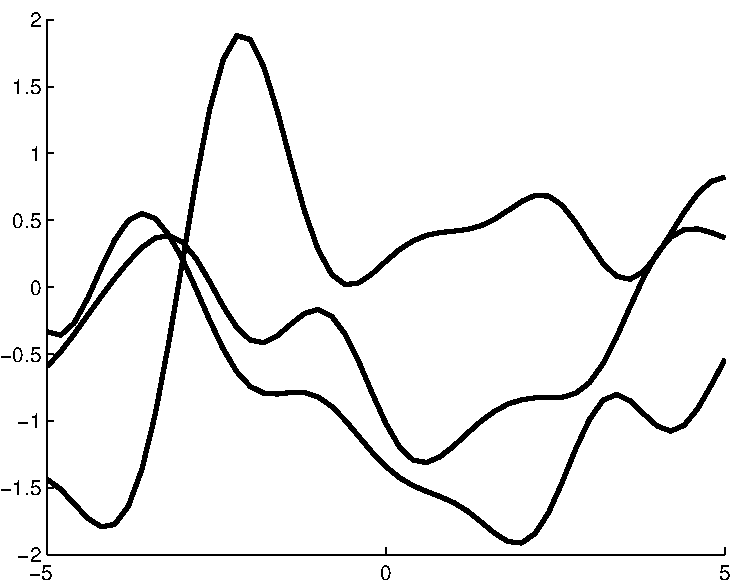
\includegraphics[width=40mm]{gprDemoNoiseFreePrior}}
\subfigure[]{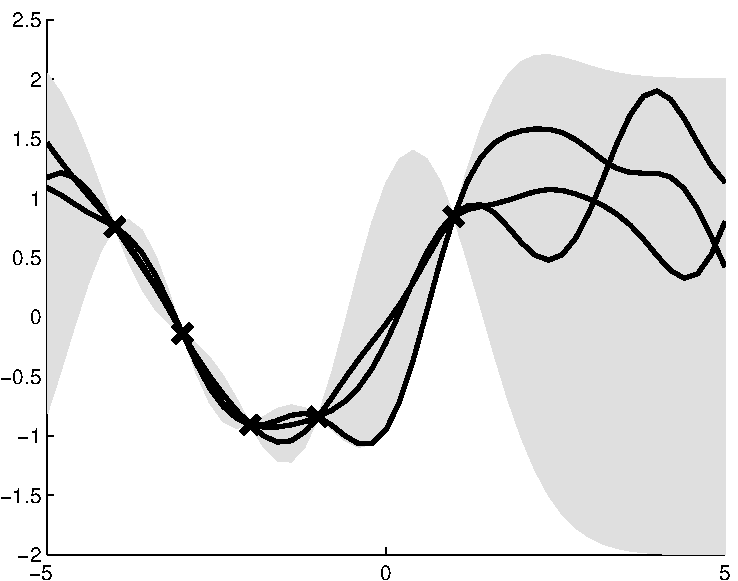
\includegraphics[width=40mm]{gprDemoNoiseFreePost}}
%\caption*{A figure}
\caption{Left: some functions sampled from a GP prior with SE kernel. Right: some samples from a GP posterior, after conditioning on 5 noise-free observations. The shaded area represents $E [f(\bm{x})]\pm2\text{std}(f(\bm{x}))$. Based on Figure 2.2 of (Rasmussen and Williams 2006). Figure generated by \texttt{GprDemo}.}
\end{figure}
\end{frame}

\begin{frame}{Predictions using noisy observations}
\begin{itemize}
    \item $y = f(\bm{x}) + \epsilon$, where $\epsilon \sim N (0, \Sigma_y^2)$.
    \item The covariance of the observed noisy responses is 
    \begin{equation*}
        \text{cov} [y_p, y_q] = \kappa(\bm{x}_p, \bm{x}_q) + \Sigma_y^2 \delta_{pq}, \quad \text{where}\quad \delta_{pq} = \mathbb{I}(p = q)
    \end{equation*}
    \item We assume the noise terms were independent.
    \item Set mean function $m(\bm{x}) = 0$. Thus, $f(\bm{x}) \sim \text{GP}(0, \kappa(\bm{x}, \bm{x}'))$
    \item Now the joint distribution is given by
    \begin{equation*}
        \begin{bmatrix}
        \bm{y}\\
        \bm{f}_*
        \end{bmatrix} 
         \sim N
        \begin{pmatrix}
            \begin{bmatrix}
            \bm{\mu}\\
            \bm{\mu}_*
            \end{bmatrix}\!\!,&
            \begin{bmatrix}
            K(\bm{X}, \bm{X}) + \sigma^2_nI & K(\bm{X}, \bm{X}_*)\\
            K(\bm{X}_*, \bm{X}) & K(\bm{X}_*, \bm{X}_*)
            \end{bmatrix}
        \end{pmatrix}
    \end{equation*}
    \item Posterior: $ p(\bm{f}_*|\bm{X}_*, \bm{X},\bm{f}) \sim N (\bm{f}_*|\bm{\mu}_*, \bm{\Sigma}_*) $
    \begin{equation*}
        \begin{split}
            \bm{\mu}_* &   = K(\bm{X}_*, \bm{X}) [K(\bm{X}, \bm{X}) + \sigma^2_n\bm{I}]^{-1}y \\
            \bm{\Sigma}_* &  = K(\bm{X}_*, \bm{X}_*) - K(\bm{X}, \bm{X}_*) [K(\bm{X}, \bm{X}) + \sigma^2n\bm{I}]^{-1} K(\bm{X}_*, \bm{X})
        \end{split}
    \end{equation*} 
\end{itemize}      
\end{frame}

\begin{frame}{Effect of the kernel parameters}
\begin{itemize}
    \item The predictive performance of GPs depends exclusively on the chosen kernel.
    \item Suppose we choose \textbf{squared-exponential} (SE) kernel for the noisy observations
    \begin{equation*}
        \kappa_y (x_p, x_q) = \sigma_f^2 \exp(- \frac{1}{2\ell^2} (x_p - x_q)^2) + \sigma_y^2 \delta_{pq}
    \end{equation*}
    \item $\ell$ is the horizontal scale over which the function changes, $\sigma_f^2$  controls the vertical scale of the function, and $\sigma_y^2$ is the noise variance.
\end{itemize}    
\end{frame}

\begin{frame}{Effect of the kernel parameters (cont'd)}
\begin{figure}[h]
\centering
\subfigure[]{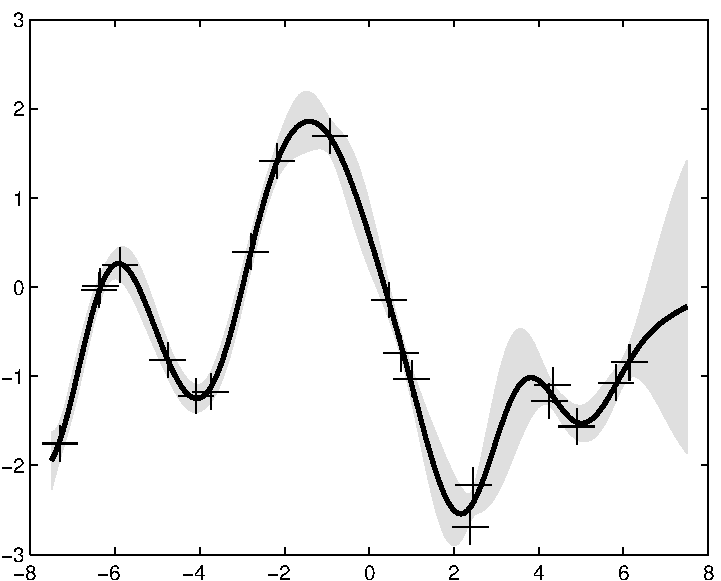
\includegraphics[width=30mm]{gprDemoChangeHparams1}}
\subfigure[]{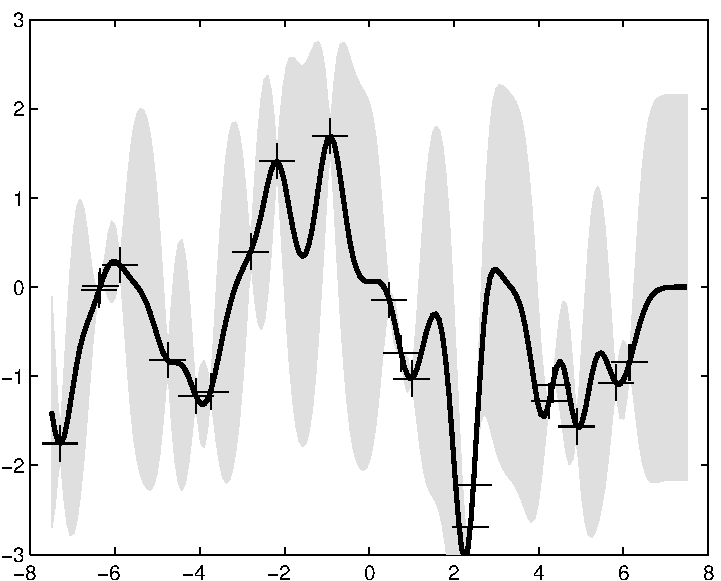
\includegraphics[width=30mm]{gprDemoChangeHparams2}}
\subfigure[]{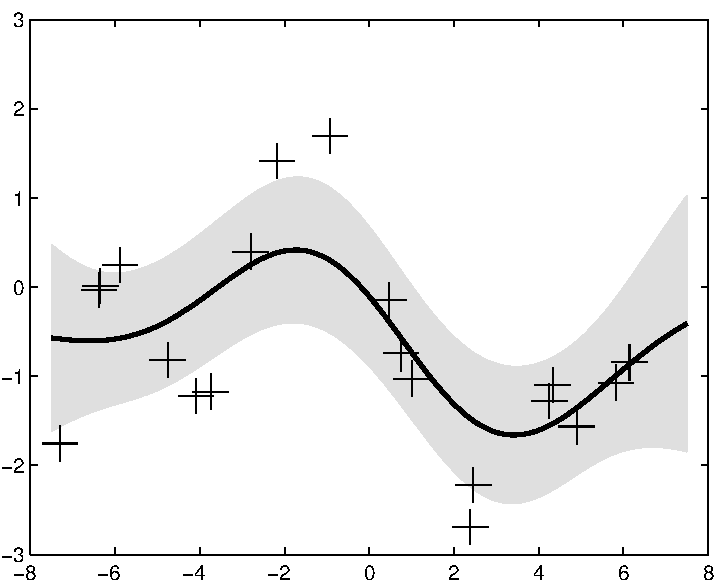
\includegraphics[width=30mm]{gprDemoChangeHparams3}}
\caption{Some 1d GPs with SE kernels but diferent hyper-parameters fit to 20 noisy observations. The kernel has the form in Equation (14). The hyper-parameters $(\ell, \sigma_f , \sigma_y)$ are as follows: (a) $(1,1,0.1)$ (b) $(0.3, 0.1.08, 0.00005)$, (c) $(3.0, 1.16, 0.89)$. Figure generated by \texttt{gprDemoChangeHparams}, written by Carl Rasmussen.}
\end{figure}
\begin{itemize}
    \item In Figure (a), the result is a good fit. 
    \item In Figure (b), the function looks more ``wiggly". Also, the uncertainty goes up faster.
    \item In Figure (c), the function looks smoother.
\end{itemize}
\end{frame}

\begin{frame}{Estimating the kernel parameters}
\begin{itemize}
    \item Frequentist: exhaustive search over a discrete grid of values (slow!).
    \item Consider empirical Bayes approach.
    \item Maximization log likelihood can be done using efficient gradient-based optimization algorithms.
    \item In absence of prior $p(\bm{\theta})$, the posterior for hyperparameter $\bm{\theta}$ is proportional to the marginal likelihood
    \begin{equation*}
        p(\bm{\theta}|\bm{X},\bm{y}) \propto p(\bm{y}|\bm{X},\bm{\theta})
    \end{equation*}
    \item Choose $\bm{\theta}$ to optimize the marginal log-likelihood
    \begin{equation*}
        \log p(\bm{\theta}|\bm{X},\bm{y}) \propto -\frac{1}{2}\log |K(\bm{X},\bm{X}) + \sigma^2\bm{I}| - \frac{1}{2}\bm{y}^T(K(\bm{X},\bm{X}) + \sigma^2\bm{I})^{-1}\bm{y}
    \end{equation*}
\end{itemize}  
\end{frame}

\section{GPs meet GLMs}
\begin{frame}{Gaussian Process Classification}
\begin{itemize}
    \item In the binary case, we have
    \begin{equation*}
        \begin{split}
            y_i & \in \{0,1 \}\\
            p(y_i|\bm{x}_i,f_i) & = \exp\{y_i f_i - A(f_i)\}\\
            p(\bm{y}) & = N(\bm{f}|\bm{0},\bm{K}), \quad \text{where} \quad K_{ij} = \kappa(\bm{x}_i, \bm{x}_j)\\
            p(y_i|\bm{x}_i,f_i) & = \text{Ber}(y_i|\text{Sigm}(f_i))\\
        \end{split}
    \end{equation*}
    \item Equivalent to logistic regression, but uses kernels rather than features.
    \item Gaussian prior on weights replaced by Gaussian prior on training log-odds.
    \item Basic inference finds MAP estimate of function $f$ at all training points
    \begin{equation*}
        \hat{\bm{f}} = \argmax_{\bm{f}}\log p(\bm{f}) + \sum_{i=1}^N \log p(y_i|\bm{x}_i,f_i)
    \end{equation*}
\end{itemize}    
\end{frame}

\begin{frame}{Gaussian Process Classification (cont'd)}
\begin{itemize}
    \item Interpretation of function values $f_i$
    \begin{itemize}
        \item \textcolor{red}{Postive:} $p(y_i = 1 |f_i) > 0.5$.
        \item \textcolor{green}{Zero:} $p(y_i = 1 |f_i) = 0.5$.
        \item \textcolor{blue}{Negative:} $p(y_i = 1 |f_i) < 0.5$.
    \end{itemize}
    \item Interpretation of kernel values $K_{ij}$
    \begin{itemize}
        \item \textcolor{red}{Postive:} likely have same label.
        \item \textcolor{green}{Zero:} inputs are totally independent.
        \item \textcolor{blue}{Negative:} likely have different labels.
    \end{itemize}
\end{itemize}    
\end{frame}

\begin{frame}{Gaussian Process Classification (cont'd)}
First, compute the distribution of the latent variable for a test case
\begin{equation*}
    p(f_*|\bm{x}_*, \bm{X}, \bm{y}) = N (\text{E}[f_*] , \text{var}[f_*]) 
\end{equation*}
Second, produce a predictive distribution for binary responses
\begin{equation*}
    \pi_* = p(y_* = 1|\bm{x}_*, \bm{X}, \bm{y}) \approx \int \text{Sigm}(f_*)p(f_*|\bm{x}_*, \bm{X}, \bm{y})df_*
\end{equation*}
\begin{itemize}
    \item Note that $p(\bm{y}|\bm{f})$ has link function involved, conjugacy of $\bm{f}$ are lost.
    \item Also integrations are difficult.
    \item \textbf{Solutions:} use analytic approximations of integrals to approximate $p(\bm{f}|\bm{X}, \bm{y})$, or Monte Carlo sampling.
\end{itemize}    
\end{frame}

\end{document}